\documentclass[a4paper, 11pt]{article}
\parskip 0.05in
\addtolength{\voffset}{-1.0cm}
\addtolength{\textheight}{2.85cm}
\addtolength{\hoffset}{-2.0cm}
\addtolength{\textwidth}{3.65cm}
\usepackage[dvips]{graphicx}
\usepackage{amsmath, amsthm, amssymb, psfrag}
\newtheorem{example}{Example} % [section]
\newtheorem{algorithm}{Algorithm} % [section]
\newtheorem{definition}{Definition} % [section]
\begin{document}


\begin{titlepage}
\begin {center}
\vspace*{0.4cm}

{\centering {\Huge Formal Methods for Accelerating Formal, Semi-formal 
	and Dynamic Property Verification through Novel Specification Styles}
\Huge \par}


%{\Large {\Huge Low Overhead Real-time \\Proportional Fair Scheduling}\Huge \par}\\
\vspace {.7in}
{\scshape  A synopsis report submitted in partial fulfillment of the requirements}\\
{\scshape for the degree of}\\
\sf
\vspace {0.4in}
{\large Doctorate of Philosophy}\\

{in}\\
{\large Computer Science and Engineering}\\
\vspace {.5in}
\large
{by}\\
\vspace{.1in}
{\bf Ansuman Banerjee} (Roll No: 04CS9701) \\
\vspace {.1in}
{under the guidance of}\\
\vspace{.5in}
{\bf Prof. Pallab Dasgupta} \\
\vspace {.1in}
{and} \\
\vspace {.1in}
{\bf Prof. P.P.Chakrabarti} \\
\vspace{.5in}
\begin{figure}[htbp]
%\centerline{\hbox {\psfig{file=Iit-25.eps,width=1.5in,height=1.5in}
{\centering \resizebox*{!}{5cm}{
\includegraphics{iit-25.eps}} \par}
%}}
\end{figure}

{
{\bf Department of Computer Science and Engineering}\\
{\bf Indian Institute of Technology Kharagpur}\\
}
\end {center}
\end{titlepage}
\newpage
\tableofcontents
\newpage

\section{Introduction} \label{sec1}
\noindent
In the past decade, the semiconductor industry has experienced a challenging 
evolution in the complexity of digital integrated circuit (IC) designs: 
increasing integration density and die size have made it possible to 
design chips with multi-million transistors. With the support of modern 
Computer Aided Design (CAD) technology, the time span
for transforming a concept to a complete product has been significantly
reduced. Industrial strength design automation tools for modeling, simulation,
synthesis and layout have now reached a fairly high level of
sophistication~\cite{synopsys_beh,dc,synopsys,vcs}. 
In this fast evolving landscape, ensuring that the designs are functionally 
correct is crucial: an error in the design's functionality can not only 
delay product deployment by months, but also lead to the loss of life (in 
safety critical applications).

Due to the increasing importance of design correctness, a significant 
fraction of 
engineering development time and resources are devoted to it~\cite{cav}. 
Design verification involves checking that the functional implementation of a 
circuit is correct against its specifications. It consists of a whole 
set of activities aiming at acquiring a reasonable certainty level that 
a design implementation will function correctly. 
Since about seventy per cent of the design cycle is spent
in validating the design, developing new methods for fool-proof verification
and integrating them in the current flow are among the biggest research
problems today.

For decades, the predominant trend in validation has been
{\em simulation and testing}~\cite{soc}. Simulation based validation 
essentially attempts to explore the possible behaviors and scenarios of the 
system with the help of a testbench that drives test vectors to the
system under test and checks for correctness. In recent times, most leading 
chip design companies are seriously investigating the possibility of 
integrating property verification into their pre-silicon validation flows. 
Property verification allows the designer to express the key
correctness requirements of a design in terms of formal properties and
verify them over a given implementation. 

Property verification is predominantly used in two forms in pre-silicon
validation, namely (a) dynamic Assertion-based Verification (ABV), and 
(b) static Formal Property Verification (FPV). In both forms, the properties 
are written in a formal specification language. ABV is a simulation-based 
approach, where the properties are checked over a simulation run -- the 
verification is thereby confined to only those behaviors that are encountered 
during simulation. FPV techniques formally verify whether {\em all} possible 
behaviors of the design satisfy the given properties. The promise of 
exhaustive validation is one of the main attractions of FPV technology. It is
unrealistic to obtain a similar guarantee through simulation driven approaches,
in view of the number of intricate directed tests that would be required to
achieve full coverage of potential behaviors. Unfortunately, FPV technology 
today does not scale beyond small circuit modules, due to its requirement 
of huge computing resources. ABV, however, being simulation-based, is scalable. 
This {\em verification crisis} has inspired a recent trend 
towards the deployment of semi-formal techniques which combine both 
formal search and simulation-based techniques in a unified setting, 
thereby, attempting to provide a scalable and more comprehensive 
validation solution.

The two main tasks for a practitioner of property verification are as 
follows:
\begin{enumerate}

\item {\em Development of the formal property specification}: The main
    challenge here is to express key features of the design intent in
    terms of a succinct and non-ambiguous formal specification. 

\item {\em Verifying the implementation against the formal property
    specification}: Considerations of scalability and comprehensiveness 
	of verification have always perplexed validation engineers in 
	choosing the verification methodology 
	and deploying it successfully in a validation project.

\end{enumerate}

\noindent
Both the tasks above are replete with open issues. In this thesis, we 
address some of these issues and propose new formal methods for accelerating 
formal, semi-formal and dynamic property verification. We believe that the 
methods presented in 
this thesis will lead to wider adoption of property verification in the 
validation flow of chip design companies.

\section{Background and Related Work} \label{sec2}
\subsection{Formal Specification Development} \label{sec2.1}
The first task in all forms of property verification is the development of
the formal specification in a formal temporal specification language. 
This is a non-trivial task and typically done by
a few specialized verification engineers today.

\subsubsection{Temporal Logics} \label{sec2.1.1}
Temporal logics were originally
developed by philosophers for reasoning about events across temporal worlds
using natural language. Pnueli was the first to use Linear Temporal Logic 
(LTL) to reason about the temporal behavior of concurrent
programs~\cite{pnueli:77}. 
In~\cite{ctl}, Clarke, Emerson and Sistla proposed the use of
Computation Tree Logic (CTL) for the specification and verification of branching
time properties. LTL and CTL are 
the most commonly used property specification logics used for formal
property specification. 
In this discussion, we explain the basic temporal operators of LTL.

The basic set of temporal operators in {\em Linear Temporal Logic} (LTL) are:
\begin{description}

\item[$X$: {\em The next-time operator}] The property, $X\varphi$, is true
    at a state of the underlying design-under-test (DUT) if $\varphi$
    is true in the next cycle, where $\varphi$ may be another temporal
    property or a Boolean property over the state bits. 

\item[$F$: {\em The future operator}] The property, $F\varphi$, is true at a
    state if $\varphi$ is true {\em sometime} (at some state) in the
    future.

\item[$G$: {\em The global operator}] The property, $G\varphi$, is true at a
    state if $\varphi$ is true {\em always} in the future.

\item[$U$: {\em The until operator}] The property, $\varphi\ U\ \psi$ is
    true at a state if $\psi$ is true at some future state, $t$, and
    $\varphi$ is true at all states leading up to $t$.

\end{description}
The operators $X$ and $U$ are the only fundamental temporal operators -- $F$
and $G$ can be derived from combinations of $U$ and Boolean operators. 
Example~\ref{ex1.1} illustrates the basic operators.

\begin{example}\label{ex1.1}
{\em Consider the specification of an arbiter that arbitrates between two 
request
lines $r_1$ and $r_2$ from two master devices. Let the corresponding grant
lines to the master devices be $g_1$ and $g_2$. The arbiter also receives
an input $z$ from a slave device, that remains high as long as the slave
device is {\em ready}.
The arbiter has the following requirements.

\begin{itemize} 
\item $A_1$: Whenever $r_2$ is asserted and the slave is ready (that is, $z$ is
high), the arbiter must give the grant, $g_2$ in the next cycle, and continue
to assert $g_2$ as long as $r_2$ remains asserted. 
\item $A_2$: When $r_2$ is not high,
the arbiter parks the grant on $g_1$ regardless of whether $r_1$ is asserted.
\item $A_3$: The request $r_2$ is fair in the sense that it
is de-asserted infinitely often.
\end{itemize}

\noindent
These requirements are expressed in LTL as follows:
\begin{tabbing}
aa \= aaaaaa \= aa \= \kill
\> $A_1$: \>
    $G(\ (\ r_2\ \land\ z\ )\ \Rightarrow\ X(\ g_2\ U\ \lnot r_2\ )\ )$\\
\> $A_2$: \>
    $G(\ (\ \lnot r_2\ )\ \Rightarrow\ X\ g_1\ )$ \\
\> $A_3$: \>
    $G\ F(\ \lnot r_2\ )$
\end{tabbing}

\noindent
This constitutes the formal specification for the arbiter in LTL.
} $\Box$
\end{example}

\noindent
Some extensions of LTL and CTL were proposed by researchers in the 
academic community over the past few decades. Some of the notables 
ones include RTCTL~\cite{Emerson:89}, TCTL~\cite{Alur:93}
and TLTL~\cite{Alur:94}.

In recent times, active participation from chip design and Electronic
Design Automation (EDA) companies have led to the adoption
of several languages for formal property specification, such as
PSL~\cite{psl} and System Verilog Assertions (SVA)~\cite{sva},
both of which are now IEEE standards. These logics derive their 
underlying semantics primarily from LTL.

\subsubsection{Consistency Issues in Specification Development} \label{sec1.2}
The first major challenge faced by every verification engineer who uses 
property verification is
to ascertain whether the specification itself is correct. Functional
correctness is very difficult to check since we do not have any formal
reference against which we may perform this verification. However it is
possible to check whether the specification is inherently consistent, or
whether there are contradictions within the specification itself. 
Detecting inconsistencies in specifications is a non-trivial task, and 
is therefore, an area of active research~\cite{pdgbook, rosner}.
In this discussion, we briefly mention three popular consistency issues 
in specification development, namely those of {\em satisfiability}, 
{\em realizability} and receptiveness. A detailed discussion on these 
issues appears in~\cite{pdgbook}.

A system property over a set of variables is {\em satisfiable} if there
exists an assignment of values to the variables in each time step such that
the property is satisfied. Consider the LTL property $X\ p \land X\ \neg p$. 
Clearly, this is unsatisfiable, while $X\ p \land F\ \neg p$ is 
satisfiable. 

To explain the concepts of realizability and receptiveness, we need the 
concept of an open system. Temporal logics like LTL and CTL were originally 
defined for closed systems, that is, systems which are self contained and 
have no external inputs. While this may be the case for a circuit as a 
whole, it is certainly not the case for the individual modules in the 
circuit which will
typically receive inputs from the other modules. A module is an
{\em open system} (e.g. arbiter in Example~\ref{ex1.1}) whose behavior is a 
function of the inputs it receives from its environment.

The semantics of properties
for open systems may be viewed as a game between the module and its
environment, where the module decides the values of the output variables and
the environment decides the values of the input variables. A property 
is {\em realizable} if a module is able to set the values of the
output variables in a way such that the property is satisfied for {\em all}
possible legal behaviors of the environment. Consider the following example.

\begin{example}
{\em
An arbiter has a high priority request input, $r$, and the corresponding
output grant, $g$. The arbiter specification (a document in English) has the
simple statement that {\em whenever the high priority device makes a request,
the arbiter must give it the grant for the next cycle}. One may be tempted
to express this requirement with the LTL property:
\[ \varphi: G(\ r\ \Rightarrow\  Xg\ \land\ XX \neg g\ ) \]

\noindent
The property formally expresses that {\em whenever
we have $r$, $g$ is asserted in the next cycle and de-asserted after one
cycle}. $\varphi$ is {\em unrealizable}, that is, there cannot exist any
implementation of the arbiter that guarantees this property. To see the
problem, consider the scenario where the high priority device requests in
successive cycles, $t$ and $t+1$. To handle the request at $t$, the
module must assign $g=0$ at $t+2$. On the other hand, to handle the request
at $t+1$, the module must assign $g=1$ at $t+2$.

The above property is {\em satisfiable} when we do not distinguish between
the input and output variables. We can then assign values to $r$ in a way
that it is not asserted in successive cycles. $\Box$
}
\end{example}

\noindent
In practice, realizability is not an adequate requirement for the
consistency of a specification. Ideally we expect a module to have
the freedom of choosing any valuation of its output variables that does not
refute the property. In some cases, a realizable specification may not
allow this freedom. Consider the following property for a module
having input $i$ and output $o$:
\[ G(\  o\ \Rightarrow\  X\ i ) \]
The property is realizable by any module that never asserts the output $o$.
The problem here is that the module needs to always assign $o=0$ because it
is unable to foresee the value of input $i$ in the next cycle. Therefore in
a given cycle, it does not have the freedom of assigning $o=1$ even though
that does not cause a refutation in that cycle. A specification that allows
the module to freely choose its outputs from those valuations that do not
cause an immediate refutation is called a {\em receptive} specification.

The notions of {\em satisfiability}, {\em realizability} and
{\em receptiveness} of temporal specifications 
have been well studied.
LTL satisfiability~\cite{vardi} has the same complexity as LTL model 
checking (PSPACE complete) and is a part of most existing model checking tools
~\cite{magellan, vis}.  Receptiveness was formalized by Dill in~\cite{dill}. 
The notion of realizability was formalized by Pnueli and Rosner
in~\cite{rosner}. It was shown that realizability checking is 
2EXPTIME-complete. The high complexity of the LTL realizability problem 
has inspired several research in this area. Some of the notable ones 
include identifying easily realizable LTL subsets~\cite{alur-ltl} to using 
game-based and simulation-based 
optimizations for easier LTL synthesis~\cite{barbara}. In a recent 
paper~\cite{nir}, Peterman
et al. have defined Generalized
Reactivity (1) (GR (1)) LTL, for which the realizability problem can be
solved in EXPTIME.

\subsection{Property Verification Approaches} \label{sec2.2}
\subsubsection{The FPV approach} \label{sec2.2.1}
The FPV setup~\cite{pdgbook} is shown in Figure~\ref{fig1.4}. At the heart of 
this approach we have a {\em model checking}~\cite{clarke:00} tool. 
A model checking
algorithm has two main
inputs -- a formal property and a finite state machine representing the
implementation. The role of the algorithm is to search all possible paths
of the state machine for a path which refutes one or more properties. If one
exists, then the path trace is reported as the {\em counter-example}. Otherwise
the model checker asserts that the property holds on the implementation.

\begin{figure}[htb]
\centering
\psfrag{p1}{\small $G[r_1 \Rightarrow  Xg_1 \land  XXg_1 ]$}
\psfrag{p2}{\small $G[ \neg g_1 \Rightarrow  g_2 ]$}
\psfrag{p3}{\small $G[ \neg g_1 \lor \neg g_2 ]$}
\psfrag{p4}{\small $G[ \neg r_1 \land  X\neg r_1 \Rightarrow XX\neg g_1 ]$}
\includegraphics[scale=0.5]{fpv.pstex}
\center
\caption{Formal Property Verification Platform} \label{fig1.4}
\end{figure}

The main limitation of model checking technology is in capacity.
Typically the main bottleneck is in the size of the FSM
extracted from the implementation. For example, the complexities of both CTL
and LTL model checking are linear in the size of this FSM.
CTL model checking is also linear in the
size of the property. LTL model checking algorithms are exponential in the size
of the properties, but there is not much of a capacity issue here, since 
typically properties are quite small in size.
The number of states in the machine typically grows exponentially with the
number of concurrent components. For designs of moderate size, this leads to
state explosion.

A lot of research in formal property verification has been on
developing solutions to combat the state explosion problem. Some of the
notable approaches are symbolic methods~\cite{mc}, bounded model checking 
(BMC)~\cite{bmc}, abstraction~\cite{dam} based methods, approximate model 
checking~\cite{approx}, ATPG-based approaches~\cite{abraham},
assume-guarantee verification~\cite{henzinger} and modular 
validation~\cite{grumberg:94}. In Section~\ref{sec6}, we present some novel 
ideas on modular validation.

\subsubsection{The Dynamic ABV approach} \label{sec2.2.2}
In the dynamic ABV approach, we write a test bench to drive inputs
into the implementation. The complexity of this task grows rapidly with the
complexity of the design. This is because the environment of a module is
typically constrained by the behavior of the other modules in the design
and by the protocol used for their communication. For example, to verify
an endpoint device in a PCI Express architecture, the test bench must model
the rest of the architecture consisting of other endpoints, the switches and
the root complex. Even after this is done, it is not practically feasible
to write directed tests to sensitize all possible behaviors of this model.

\begin{figure}[htb]
\centering
\includegraphics[scale=0.5]{diag2.pstex}
\center
\caption{Assertion-based Verification Platform} \label{fig1.2}
\end{figure}

The dynamic ABV setup is shown in Figure~\ref{fig1.2}. We simulate the
implementation with the test bench. The assertion checker reads the signals in
the interface and monitors the status of the properties. If any of the
properties fail during the simulation, the checker reports it immediately. The
failure points help the verification engineer to isolate the source of the bug.

There are two key features of dynamic ABV which explain the 
popularity of this approach. Firstly, it is built over the
traditional simulation framework and requires nominal additional effort
from the verification engineer. Secondly, it does not have any major capacity
concerns, since the verification is done over the simulation run.

The main criticism of this approach is that the fraction of the design 
space which can 
be explored by simulation is miniscule, especially for large designs. 
Only one state and one input combination of the design under test 
are visited during each simulation cycle. Moreover the test stimuli 
are hand crafted by the designer to cover those areas of the design 
that he wishes to validate. For a large, complex system, it is 
impossible to test or simulate all possible inputs or sequences 
of inputs. Furthermore, simulation inputs are usually based on the design 
specification and are thus only aimed at verifying that the design 
performs all the primary activities indicated in the specification 
document. However, it is often the case that complex systems manifest 
unforeseen behavior for corner case situations. Most often, designers 
are unaware of behavior that results as a by-product of the interactions 
among different modules and that was unaccounted for in the specification 
document. These cases do not get checked, while they may have 
negative consequences on the overall behavior of the system.

In view of the volume of directed tests that needs to be written in order to
achieve a meaningful level of functional coverage, the industry is moving
towards coverage driven randomized test generation~\cite{rvm}. This helps 
in reaching
a high level of coverage in short time, but the difficult corner case
behaviors are typically left out. Formal properties target these
corner case behaviors, but dynamic ABV is not effective unless we can force
the test bench to create the relevant scenarios.

Much research~\cite{ammann, garg, SAT:01} in the validation community has 
been carried out to define an automated methodology for generating tests 
from formal specifications. These include methods for defining special 
constructs for characterizing the input space~\cite{clarke:00a}, 
offline monitoring~\cite{tasiran}, counterexample-guided test 
generation~\cite{ammann} and ATPG-based approaches~\cite{abraham}.
In Section~\ref{sec4}, we present our contribution in this direction.

\subsubsection{Semi-Formal Verification} \label{sec2.2.3}
The past few years have witnessed the emergence of a range of 
semi-formal verification approaches, which attempt to combine the 
advantages of formal and simulation-based techniques in a unified 
setting. This has found better success in design 
validation in uncovering deeply rooted bugs, which manifest themselves 
only in specific corner case scenarios (and may therefore be missed by 
simulation) and require sufficient expansion of the design 
hierarchy (which renders FPV unsuitable).

The key motivation behind many of these semi-formal approaches is 
to localize the formal search over those behaviors that are targeted by
corner case scenarios. A survey~\cite{guido}
of these approaches shows that a wide range of techniques, ranging from
theorem-proving and abstraction-guided counterexample
search to symbolic/logic simulation and ATPG-based methods have been
employed. In~\cite{guido}, the authors present an
approach that uses formal verification techniques to guide simulation
towards a verification goal, based on an abstract model of the design.
In~\cite{kunz}, Kunz et al present a method for extracting
reachability constraints to avoid false negatives in a BMC setting. 

\section{Contributions of this dissertation} \label{sec3}
The benefits of property verification have been established quite 
emphatically in the last decade. Researchers have analyzed several 
historically significant failures and have shown that the use of property 
verification could have detected the bug in the design.
Yet, there has not yet been sufficient penetration of property verification 
techniques into the validation flow of chip design projects. For the 
software community, the success has been even less, and software property 
verification is still at a premature state of deployment. 

To improve the overall scenario, we need efficient methods that can 
enable property verification penetrate the validation flow of 
a larger cross-section of companies. This thesis is an attempt in that
direction. In this thesis, we propose new formal methods 
for accelerating formal, semi-formal and dynamic property verification.
Specifically, this thesis has the following contributions:
\begin{enumerate}
\item {\bf Property guided simulation for dynamic ABV:}
	The main criticism of the dynamic ABV approach is that only those 
	behaviors that are covered by simulation are examined for property 
	violation. The first contribution 
	of this thesis is to define an automated methodology that can analyze 
	formal properties and produce tests that trigger them. These tests 
	are used to guide simulation, thereby resulting in higher assertion 
	coverage and better verification productivity. The simulation is 
	carried out using a novel online constraint satisfaction approach. 
	Our algorithm has been 
	integrated within the layered verification methodology of RVM~\cite{rvm} 
	with significant improvement in assertion coverage as compared to 
	a coverage-driven randomized verification approach.

\item {\bf Context-Sensitive Formal Specifications:} A significant fraction 
	of the 
	correctness requirements in standard protocol descriptions are relevant 
	in particular contexts of the protocol. Property specification languages 
	alone are not convenient enough for modeling such {\em context-sensitive} 
	requirements. In this thesis, we have formalized a specification 
	modeling style consisting of abstract {\em context state machines} and 
	context-sensitive properties, and examined the following problems:

\begin{itemize}
\item {\bf FPV with Context-Sensitive Formal Specifications:} We have shown 
	that 
	specifications consisting of auxiliary context state machines and 
	context-sensitive formal properties in Linear Temporal Logic can 
	lead to significant computational advantages in model checking. 
	This is an important news for deployment of FPV in design validation, 
	considering the fact that a large percentage of common correctness 
	requirements are context-sensitive. 

\item {\bf Semi-Formal Verification with Context-Sensitive Formal 
	Specifications:}
	We have developed a semi-formal verification approach for verifying 
	this style of specification, using a mix of property guided simulation 
	and bounded model checking. The proposed methodology has been integrated 
	with Magellan~\cite{magellan} and VIS~\cite{vis}, with dramatic 
	improvement in performance -- both in terms of speed and scalability.

\item {\bf Consistency Analysis of Context-Sensitive Formal Specifications:}
	We have examined the complexities of the satisfiability and 
	realizability of formal specifications in this mixed specification 
	style. In addition, we have shown that formal specifications 
	consisting of auxiliary state machines and context-sensitive 
	formal properties restricted to the GR(1)~\cite{nir} fragment of 
	LTL entails a EXPTIME realizability checking procedure.
\end{itemize}
\item {\bf Open Linear Temporal Logic (Open-LTL):} To ameliorate the 
	state explosion
	problem, there has been a paradigm shift from a system level FPV  
	perspective to a modular one. Popular temporal logics like LTL were 
	originally defined for closed system level specifications, and 
	admit a lot of specification inconsistencies when interpreted over 
	modules. We have formalized an extension of LTL that is suitable for 
	formal specifications at the modular level. In addition, we have shown 
	that the proposed style can be easily integrated with traditional 
	FPV algorithms and developed a complete in-house tool suite for 
	modular validation.

\item {\bf An integrated framework for ABV for UML Statecharts:} In the 
	software verification community, the Unified Modeling Language 
	(UML)~\cite{uml}
	is being extensively used as a formalism for design of large 
	safety critical systems. We have developed an integrated framework 
	for dynamic property verification of Statechart based designs in UML. 
	The main contribution has been the formalization of an extension 
	of LTL, namely Action-LTL for specification of formal properties 
	over state-event systems, and a methodology for ABV of Action-LTL 
	properties over UML models. Our methodology has been integrated 
	within an industry standard tool, Rhapsody~\cite{rhap}, popularly used 
	for model driven 
	development for UML. We believe the successful deployment of ABV over 
	Rhapsody achieved by us in this work will open up the avenue for 
	future research on ABV for more generic software validation.
\end{enumerate}

\noindent
In the following sections, we illustrate on each of the above contributions. 

\section{Property Guided Simulation for ABV} \label{sec4}
In this section, we present our approach for generation of test vectors 
that can guide simulation when the goal is to cover a given set of properties. 
Fundamentally, the problem of automatic test generation for covering assertions
may be formulated as a game between the design-under-test (DUT) module 
and its environment (that is, the
test generator). This is because of the fact that the test generator has no
control over the behavior of the DUT. In other words, the DUT is a black-box
-- we can drive inputs into it, but we can neither predict, nor influence its
behavior in any way. The winning objectives in this game are different 
for each of the two players. At each cycle, the DUT attempts to satisfy a given 
property by setting appropriate values to its outputs, where as the test 
bench attempts to refute it by controlling the input signals. The module and 
the test bench alternate over time. The module has a bug if the test bench has a
strategy to refute the property.
An intelligent test bench must be online and adaptive, and should have the
following two features:

\begin{itemize}

\item The test bench should avoid generation of input vectors satisfying 
      the specification {\em vacuously}.

\item If at any point, the module produces an output that may lead to
      failure under some specific input scenario, then the test bench should
      drive that scenario to lead the module to failure, and
      expose the bug. This may happen over multiple cycles.

\end{itemize}

\noindent
In the following subsections, we illustrate on each of the above.

\subsection{Non-vacuous Input generation} \label{sec4.1}
\noindent
In this section, we first address the issue of vacuity
in test generation for verification of modules. Consider the following 
example.

\begin{example} \label{example1}
{\em
Consider an arbiter A, having two input request lines, $r_1$ and $r_2$,
and three grant lines, $g_1$, $g_2$ and $g_d$. The functionality of
the arbiter is described as below:

\begin{enumerate}
\item Whenever $r_1$ goes high, $g_1$ is asserted in the
        next cycle. \\
	  $P_1$: $\ G(r_1\  \Rightarrow\ Xg_1)$
\item Whenever $r_2$ goes high, $g_2$ is asserted within
        3 cycles. \\
      $P_2$: $\ G(r_2\  \Rightarrow\ Xg_2\ \lor\ XXg_2\ \lor\ XXXg_2)$
\item $g_d$ (default slave grant) is asserted at least once in every 3 cycles.\\
	  $P_3$: $\ G(g_d\  \lor\ Xg_d\ \lor\ XXg_d)$
\item The grant lines are mutually exclusive. \\
	  $P_4$: $\ G(mutex(g_1,\ g_2,\ g_d))$
\item The request lines $r_1$ and $r_2$ are mutually exclusive. \\
	  $A_1$: $\ G(mutex(r_1, r_2))$
\item The request $r_1$ never arrives in successive cycles.\\
	  $A_2$: $\ G(r_1\  \Rightarrow\ X \neg r_1)$
\item When $r_2$ arrives, it remains high until $g_2$ is asserted. \\
	  $A_3$: $\ G(r_2\  \Rightarrow\ (r_2\ U\ g_2))$
\end{enumerate}
The last 3 properties are assumptions on the arbiter inputs.
%\begin{enumerate}
%\item $P_1$: $\ G(r_1\  \Rightarrow\ Xg_1)$
%\item $P_2$: $\ G(r_2\  \Rightarrow\ Xg_2\ \lor\ XXg_2\ \lor\ XXXg_2)$
%\item $P_3$: $\ G(g_d\  \lor\ Xg_d\ \lor\ XXg_d)$
%\item $P_4$: $\ G(mutex(g_1,\ g_2,\ g_d))$
%\item $A_1$: $\ G(mutex(r_1, r_2))$
%\item $A_2$: $\ G(r_1\  \Rightarrow\ X \neg r_1)$
%\item $A_3$: $\ G(r_2\  \Rightarrow\ (r_2\ U\ g_2))$
%\end{enumerate}
\noindent
The objective of ABV is to check whether the arbiter satisfies the
properties $P_1, \ldots, P_4$ in those simulation runs that
satisfy the {\em assume constraints}, $A_1, \ldots, A_3$. Simulations
refuting one or more of these assume constraints are invalid,
not because the arbiter has a bug, but because the test bench
drives invalid input sequences. The first responsibility of a test
bench is to drive input sequences that satisfy all assumptions.

Even when an input sequence satisfies all assume constraints, it may
not {\em trigger} a given property. For example, consider an input
sequence where $r_2$ is never asserted. This sequence satisfies
all assumptions, but does not trigger the property $P_2$.
To create the meaningful scenarios for which $P_2$ was
written, the test bench must drive input sequences where $r_2$
is asserted. The input sequences which trigger a property constitute the set 
of environment strategies for which the module behavior must be validated. 
The challenge is in creating such non-vacuous tests.
}$\Box$
\end{example}

\noindent
As demonstrated in the above example, the test generator must always
generate tests that are non-vacuous with respect to the set of properties.
The requirement of non-vacuity is not limited to a particular cycle, and
may span multiple cycles as well, over different input vectors.
Consider the following example specification for a IBM-CoreConnect~\cite{ibm}
compliant PLB Master device:

\begin{example}
{\em The PLB Master should assert ReadBurst signal for the
secondary acknowledged burst read transfer in the
following cycle after receiving ReadBurstTerm from the Slave device for the
on-going primary burst read transfer. The LTL property is:
{
\begin{tabbing}
aa \= aaa \= aaa \= aaaa\= aaaaa\= \kill
$\psi$: $G(((ReadBurst \land PAV \land S\_Ack) \land X(ReadBurst \land SAV \land$ \\
\>\> $S\_Ack) \land XX (ReadBurstTerm)) \Rightarrow XXX(ReadBurst))$
\end{tabbing}
}
\noindent
To test the above property for a PLB master device in isolation, the signals
PAV, SAV, S\_Ack, and ReadBurstTerm (which are inputs to the PLB master)
should be driven from the test bench. A purely random test bench in reasonable
time would fail to create such a complicated pre-condition spanning over 3
cycles (in the first, $PAV \land S\_Ack$, in the next,
$SAV \land S\_Ack$, followed by
$ReadBurstTerm$ should be driven). However, to test this property,
a test bench should create this corner case scenario.
}$\Box$
\end{example}

\noindent 
The following definition formalizes the concept of a {\em vacuous input 
vector} with respect to a property.
\begin{definition} {\bf [Vacuous input vector]}\\
{\em 
An input vector, $\widehat{I}$, is vacuous at a given step with respect to a
property, $\varphi$, iff $\varphi$ becomes true at that step on input
$\widehat{I}$ regardless of the values of the remaining variables. $\Box$
}
\end{definition}

\noindent
For each property, our target is to drive a sequence of input vectors
such that a non-vacuous success/failure of the property is reported.
Therefore, we
define our coverage points as non-vacuous interpretations of {\em individual}
properties and create tests that target each coverage point in turn.
Consider the following example.

\begin{example} \label{egvac}
{\em Consider the specification ${\cal Q}$ for a priority arbiter
having inputs $r_1$, $r_2$ and outputs $g_1$, $g_2$. ${\cal Q}$
contains the following properties:
\begin{enumerate} 

\item Whenever $r_1$ remains high for two consecutive cycles, $g_1$ should
    be asserted in the next cycle. \\
    $Q_1$: $G(r_1\  \land Xr_1 \Rightarrow\ XXg_1)$
\item Whenever $r_2$ goes high, with $r_1$ remaining low, $g_2$ must be
    asserted in the next cycle. \\
    $Q_2$: $G(r_2\  \land\ \neg r_1\ \Rightarrow\ Xg_2)$
\end{enumerate}
We want to test both $Q_1$ and $Q_2$ non-vacuously. These are
our coverage points. For $Q_1$, the test bench must drive
$r_1 = 1$ and choose $r_2$ randomly for two consecutive cycles.
For $Q_2$, it must drive $r_2 = 1$ and $r_1 = 0$. Note that in the
first case, $Q_2$ is satisfied vacuously, while in the second case
$Q_1$ is satisfied vacuously.
} $\Box$
\end{example}

\subsection{Test generation for unreceptive specifications} \label{sec4.2}
A common problem in dynamic ABV
with temporal specifications is that the property
refutation may happen several cycles after the actual fault. This is typically
the case for unreceptive specifications~\cite{dill}. Moreover,
the refutation may depend on the inputs that are driven after the
fault. Consider the following example:

\begin{example} \label{example3}
{\em Consider the scenario shown in Fig~\ref{timing} for 
Example~\ref{example1}.
At time $t$, the grant was parked on $g_d$ and $r_1$ was asserted.
At $t+1$, the arbiter asserted $g_1$ (satisfying $P_1$), and the test
bench raised $r_2$. At $t+2$, the arbiter asserted $g_2$, and the
test bench raised $r_1$. At this point, a failure is imminent at
$t+3$ because $P_1$ requires $g_1$ to be raised, $P_3$ requires
$g_d$ to be raised, and $P_4$ disallows both $g_1$ and $g_d$ high.

\begin{figure}[htb]
\centering
\includegraphics[scale=0.66]{diag43.pstex}
\caption{A Conflicting Scenario} \label{timing}
\end{figure}

Here, the fault occurred at $t+2$ when the arbiter asserted
$g_2$. The correct behavior would have been to assert $g_d$ at
$t+2$ and then assert $g_2$ at $t+3$.
It is interesting to note that the fault would have passed undetected
had the test bench not raised $r_1$ at $t+2$. {\em Can the test
bench intelligently detect such cases and drive the appropriate
inputs to reach a refutation in some future state?} Indeed it can
by using the notion of {\em realizability} of specifications.

It is also interesting to note that though the fault occurred at $t+2$,
the specification was not refuted at $t+2$. This is a typical scenario
in {\em non-receptive}~\cite{dill} specifications. Non-receptive
specifications occur because identifying a property for every individual
scenario is  difficult in practice. For example, to detect this
fault at $t+2$, we may add the property
\[ G((r_1\ \land\ Xr_2)\ \Rightarrow\ XXg_d) \]
This is non-intuitive, unless the above scenario is
demonstrated. The property is redundant formally, since it is possible
to detect the fault at $t+2$ using a realizability checker~\cite{lily}.
}$\Box$
\end{example}

\noindent
In order to adequately address the above issue, the test generation
algorithm must be aware of the notion of realizability as given in 
Section~\ref{sec2}. A specification may be realizable
at the beginning of simulation, but when a fault occurs (that is, the
module makes a wrong move), the specification may become unrealizable but not
unsatisfiable. In other words, the property has not yet been refuted, but
we are guaranteed to drive the module to a
state where the property is refuted. This is a very important requirement,
since our end goal is to expose bugs. In Example~\ref{example3}, the
specification was realizable at time $t$. At $t+2$, when the arbiter
asserted $g_2$, the effective specification contains the property
\[ Xg_d \land (r_1 \Rightarrow  Xg_1) \land mutex(g_1, g_2, g_d) \]
which is satisfiable (consider $r_1 = 0$),
but unrealizable, because the test bench has a winning strategy
(by setting $r_1 = 1$).

Given an unrealizable specification, the goal of the test generator is to
drive the module to a state where the specification is refuted. This may
happen in a sequence of steps (with alternate moves between the module and the
test generator). In each step, the test generator needs to make sure that
the inputs generated by it does not make the specification realizable. This
game between the module and its test bench is called a {\em realizability}
game. When the module produces a fault that renders the specification
unrealizable (but not unsatisfiable), then we start a {\em realizability game}
to drive the module to a refuting state.

\subsection{Test Generation Algorithms} \label{sec4.3}
In order to address the above objectives, we have developed a 
novel test generation algorithm, which is augmented with the notions 
of realizability and vacuity of system specifications. This makes 
our approach radically different from specification-directed test generation 
approaches proposed in literature~\cite{ammann, garg, SAT:01}, since none 
of these address the issues of vacuity and realizability.

In a normal situation, at the start of each simulation cycle, the generation
of a non-vacuous input is the primary objective of our test generator, while 
it starts the realizability game when the module makes a wrong move. The 
test generation is 
done using an online monitoring approach, and is therefore, adaptive.
The details of this algorithm is given in the thesis. 

\subsection{Implementation and Results} \label{sec4.4}
The procedure of property driven test generation 
was integrated within the layered verification architecture of 
RVM~\cite{rvm} and deployed on several verification
IPs for standard on-chip Bus protocols. Our test generation algorithms
reached several complex coverage points in significantly less time
as compared to a coverage driven constrained random verification
approach. Table~\ref{tab1} shows the result of our tool for an industry
standard ABV IP for the IBM CoreConnect BUS protocol~\cite{ibm}.
It has $3$ buses, namely DCR, OPB and PLB. For each BUS we have
a number of properties, a Bus functional model, and a VM-compliant~\cite{vmm}
coverage driven random (CDR) test bench. We present the
results for a selected subset of the properties, which has complicated
triggering conditions spanning multiple cycles.

\begin{table}[!t]
\begin{center}
{\small
\begin{tabular}{|c|c|c|c|c|c|} \hline
Device    & \# Inp.    & \# Outp. & \#Prop. & IABV & CDR   \\
\hline %\multicolumn{5}{|c|}{PCI master interface} \\ \hline
\multicolumn{6}{|c|}{DCR interface} \\ \hline
master & 4 & 2 & 2 & 5000 & 7000 \\
slave  & 2 & 4 & 2 & 5400 & 8600 \\
\hline
\multicolumn{6}{|c|}{OPB interface} \\ \hline
master  & 6 & 6 & 2 & 6400 & 9200 \\
slave   & 5 & 4 & 2 & 6200 & 10800 \\
\hline
\multicolumn{6}{|c|}{PLB interface} \\ \hline
master  & 7 & 5 & 2 & 1000 & 6000 \\
slave   & 6 & 8 & 1 & 3000 & 4000 \\
\hline
\end{tabular}
}

\end{center}
\caption{Results on IBM CoreConnect} \label{tab1}
\end{table}

The last two columns of Table~\ref{tab1}
compare the number of simulation cycles required to cover all properties
non-vacuously using our tool (IABV) with that of the coverage-driven
random (CDR) one. Results show that the 
coverage improved dramatically when using our approach.

\section{Context Sensitive Formal Specifications} \label{sec5}
An analytic study of the formal specifications for a
multitude of protocols (including ARM AMBA, Hyper Transport,
IBM CoreConnect) has led us to believe that formal specifications of 
interface protocols mostly consist of two types of
correctness requirements, namely (a) a set of invariants
that applies throughout the protocol execution and (b) a set of
{\em context-sensitive} properties that applies only when the protocol is in a
specific set of contexts (bus acquisition context, transfer context etc.)
For example,
the mutual exclusion property for an arbiter (which specifies that
the arbiter issues one grant at a time) is an invariant property,
whereas a property which specifies that successive addresses must
wrap around 2KB address boundaries maybe applicable only in the
context of burst transfers (and not in general). For properties
of the second type, we need to model the context, which is not
easy in terms of formal property languages since in many cases,
the context cannot be defined in terms of the current signal
values and depends on the history of the protocol. In our
experience, context-sensitive properties account for a large
percentage of the properties in complex protocols. 

In order to facilitate the development of context-sensitive
properties, researchers~\cite{pdgbook,dill1} have
suggested the use of {\em auxiliary state machines} to model the abstract 
states of the protocol. These state machines become part of the formal
specification and significantly ease the development of
context-sensitive properties, which can now use the states
of the auxiliary state machines to define the context of the
property. The auxiliary state machines typically contain a
small subset of the DUT interface signals, whose valuations are
needed to characterize the major protocol contexts and the
context switches. This keeps them small and simple. We explain the 
advantages of this style of specification with the following example.

\begin{figure}[htb]
\centering
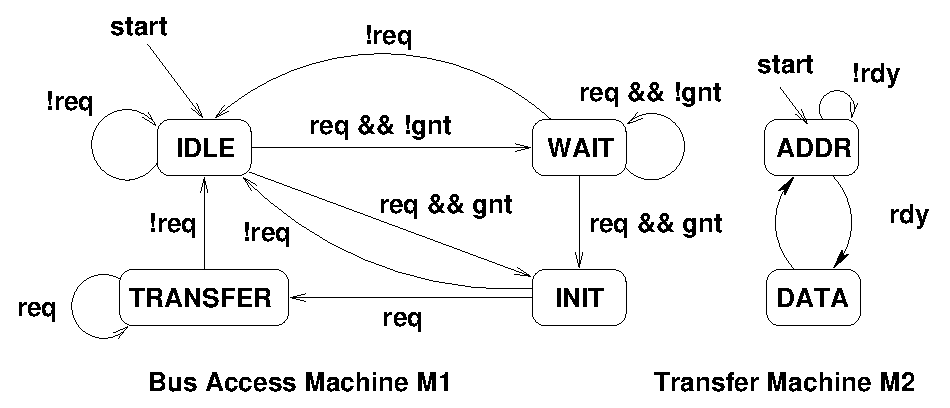
\includegraphics[scale=0.7]{diag217.eps}
\caption{Auxiliary State Machines} \label{fig1.1}
\end{figure}

\begin{example} \label{eg1}
{\em Consider the specification of a master interface participating in a 
simple bus
protocol with an arbiter and a slave device. Fig~\ref{fig1.1} shows two
auxiliary
state machines for describing the macro states of the protocol. $M1$ describes
the state of the master during bus access in terms of {\em req} (request to
arbiter) and {\em gnt} (grant from arbiter). $M2$ describes a more detailed
state
of the master during the transfer using the signal {\em rdy} (slave ready). 
Note that the auxiliary state machines involve a small fragment of the DUT 
interface signals. For our master interface, there are other signals, namely,
(a) {\em rw} (indicating the nature of current transfer, write or a read),
(b) {\em validaddr} (flag indicating the validity of the address floated on the bus)
(c) {\em abort} (transfer terminated by the slave), and
(d) {\em delayed} (delayed transfer).

The specification of the master (DUT) includes the following properties:
\begin{itemize}

\item ${\cal P}_0$: If the transfer waits due to non-availability of slave
        while
        the abort signal is low, then the delayed signal should be asserted 
		in the next cycle.
\item ${\cal P}_1$: If the master is in the ADDRESS cycle in a write transfer,
        it should always hold a valid address in the next cycle.

\end{itemize}

\noindent
Both properties are context-sensitive. ${\cal P}_0$ applies only when the 
master is in the waiting phase, whereas ${\cal P}_1$ applies only when the 
master is in
the ADDRESS phase. It is easy to code these properties using the auxiliary
state machines, as shown below:
\begin{itemize}
\item ${\cal P}_0:$ G(WAIT $\land \neg$ abort $\Rightarrow$ X\ delayed)
\item ${\cal P}_1:$ G(TRANSFER $\land$ ADDR $\land$ rw $\Rightarrow$ X validaddr)
\end{itemize}

\noindent
Let us now consider the task of developing the same properties without using
the auxiliary state machines. The main problem here is that the context states
(such as WAIT, TRANSFER and ADDR) cannot be characterized by Boolean 
propositions
over the interface signals, and require an encoding of the history of the
protocol. For example, one might be tempted to express ${\cal P}_1$ as:
\[G((req \land gnt) \land X(req \land rdy \land rw)\Rightarrow XX validaddr) \]

\noindent
The antecedent part of the implication attempts to express the context
TRANSFER $\land$ ADDR. In this form the antecedent appears non-intuitive.
Moreover the antecedent does not capture those scenarios where the DUT
reaches the TRANSFER state after stuttering in one or more WAIT states.
It is easy to see that a more accurate encoding of all possible history
will make the antecedent almost unreadable and prone to coding errors.
} $\Box$
\end{example}

\noindent
It is important to note that auxiliary state machines are developed
independently by the verification engineer as an integral part of the
formal specification -- they are not part of any given implementation,
nor are they extracted out of one. This makes our approach different from 
those in~\cite{kunz, guido}. Also protocol specs often provide
such abstract state machines (for example, see the ARM AMBA~\cite{ahb} 
protocol specs).

\subsection{The Formal Model} \label{sec5.1}
\noindent
Formally, we define a DUT module ${\cal J}$ =
$\langle {\cal I}, {\cal O}, Init, {\cal B} \rangle$ as a design block having
a set of inputs ${\cal I}$, a set of outputs ${\cal O}$, an initial block
$Init$, and a behavior ${\cal B}$ specified as RTL code.

A context-sensitive property is defined over a set ${\cal M}$ of auxiliary
state machines, each of the form $M_i$ =
$\langle {\cal I}_i, {\cal O}_i, {\cal S}_i, {\cal S}^0_i, {\cal T}_i \rangle$, where:
\begin{itemize}
\item ${\cal I}_i \subseteq\ {\cal I}$ is the set of input
    signals used in ${\cal M}_i$,
\item ${\cal O}_i \subseteq\ {\cal O}$ is the set of output
    signals used in ${\cal M}_i$,
\item ${\cal S}_i$ is the set of contexts (states) of ${\cal M}_i$,
\item ${\cal S}^0_i$ is the start context (state) of machine ${\cal M}_i$,
\item ${\cal T}_i: {\cal S}_i \times 2^{{\cal I}_i \cup {\cal O}_i}
    \rightarrow {\cal S}_i$
    is the next-state function for ${\cal M}_i$ (the transition function
    is total and deterministic,
    i.e. for every context and for every combination of
    ${\cal I}_i \cup {\cal O}_i$, there is a unique next state). We
    denote a {\em transition}
    $t$ = $T_i(s, \eta)$, where $s,t \in {\cal S}_i$ and $\eta \in
    2^{{\cal I}_i \cup   {\cal O}_i}$ by the ordered pair (s,t).
\end{itemize}

\begin{definition} {\bf [Context-Sensitive Property: ]} \label{def5.1}
A context-sensitive property is an LTL
property over ${\cal I} \cup {\cal O} \cup \bigcup_i {\cal S}_i$.
$\Box$
\end{definition}

\begin{example} \label{eg2}
{\em Consider the master specification of Example~\ref{eg1}.
${\cal I} = \{gnt, rdy, abort\}$,
and ${\cal O} = \{req, rw, validaddr, delayed\}$. The auxiliary state machine
$M_1$ has ${\cal I}_1 = \{gnt\}$ and ${\cal O}_1 = \{req\}$, while
$M_2$ has ${\cal I}_2 = \{rdy\}$ and ${\cal O}_2 = NULL$.
${\cal S}_1$ = $\{IDLE, WAIT, INIT, TRANSFER \}$, and
${\cal S}_2$ = $\{DATA, ADDR \}$, with ${\cal S}^0_1$ = $IDLE$ and
${\cal S}^0_2$ = $ADDR$.
${\cal P}_0$ and ${\cal P}_1$ are context-sensitive.
} $\Box$
\end{example}

\noindent
The advantage of using auxiliary state machines and context-sensitive 
formal properties is quite evident from Example~\ref{eg1}. In the 
following discussion, we explain the advantages of this specification 
style in verification.

\subsection{Context-Sensitive Assertions: The FPV Advantage} \label{sec5.2}
Context-Sensitive assertions have significant advantages in formal 
property verification. The intuitive reason behind this is the fact that,
we need to verify a context sensitive property only within the DUT
states that satisfy the context of the property. As a consequence, DUT 
behaviors that do not model the context can be pruned. Consider the 
property ${\cal P}_0$ in Example~\ref{eg1}. To verify this property 
non-vacuously, we need to consider only those regions of the DUT behavior 
that model the $WAIT$ context. For ${\cal P}_1$, we need to restrict 
ourselves to the DUT states which model the ADDR phase of an ongoing 
transfer. We utilized this idea to develop a symbolic verification 
algorithm based on partitioned transition relations.
The key steps of our verification algorithm for verifying a 
context-sensitive formal property are as follows:
\begin{itemize} 
\item We compute a selective composition of the auxiliary state machines, 
	based on the contexts appearing in the formal property\footnote{This 
	composition is not expensive, since each auxiliary state machine 
	typically contains a few states.}. For example, to verify ${\cal P}_0$, 
	we do not require to compose, while ${\cal P}_1$ involves context
	variables from each of the auxiliary state machines, and therefore, 
	requires the composition.
\item The composed state machine is pruned with respect to the 
	context of the context-sensitive formal property. 
\item The reduced state machine is then used to
	constrain the state space of the DUT such that
	only those parts that are relevant to the property are retained.
\item The context-sensitive property is then checked on this reduced 
	DUT using a standard LTL model checking algorithm~\cite{clarke:00}.
\end{itemize}

\noindent
The detailed algorithm behind each step above is present in the thesis, 
and not included here. Our approach has significant gains in terms of 
capacity. We implemented our methods into a tool called Context-Sensitive 
Assertion 
Verifier (CSAV). To give an idea of the comparative space utilization, 
we present a snapshot of the results obtained by us on some benchmark 
examples using our methodology as compared to a standard LTL model 
checker. 

\begin{table*}[htb]
\begin{center}
{\small
\begin{tabular}{|c|c|c|c|c|c|} \hline
Ckt. & Peak BDD & Time(s) & \# Prop. & Peak BDD & Time (s) \\
Module & size(VIS) & (VIS) & & (CSAV) & (CSAV) \\ \hline \hline
\multicolumn{6}{|c|}{IFetch} \\ \hline
IFetchControl   & 362810 & 6.9 & 10 & 263676 & 5.1    \\ \hline \hline
\multicolumn{6}{|c|}{Cache Coherence Protocol} \\ \hline
Coherence       & 143080 & 3.5 & 4 & 45990 & 2.1 \\ \hline \hline
\multicolumn{6}{|c|}{MPEG} \\ \hline
Parsepack      & 7154 & 0.6 & 2 & 7154 & 0.4 \\ \hline \hline
\multicolumn{6}{|c|}{P6bus} \\ \hline
Multimaster    & 265720 & 5.3 & 6 & 147168 & 1.9 \\ \hline \hline
Singlemaster   & 90958 & 3.3 & 4 & 73458 & 3.3 \\ \hline \hline
\end{tabular}
}
\end{center}
\caption{Results on Benchmark circuits} \label{tab2}
\end{table*}

Table~\ref{tab2} shows the results of our tool. The $2^{nd}$ and 
$3^{rd}$ 
columns show the peak BDD size (number of nodes) and time (in seconds)
obtained when the properties (Column 4) were verified using
VIS. The peak bdd size encountered by our tool for
verification and the corresponding times are shown respectively in
Columns 5 and 6. Results show the effectiveness of our approach.

\subsection{Semi-Formal Verification with Context Sensitive Assertions} 
	\label{sec5.3}
In this subsection, we briefly explain a semi-formal verification approach 
for verifying
context-sensitive properties. The semi-formal methodology proposed by us was 
motivated by the fact that in many cases, the truth of a context
sensitive property depends not on {\em how the DUT reached the context},
but on {\em what the DUT did after reaching the context}. In such
cases we achieve satisfactory (though not exhaustive) coverage by
reaching a context-satisfying state using semi-formal means and then
using a formal method to verify the property from that state. Since
the contexts are explicitly specified in terms of the auxiliary state
machines, we can use the auxiliary state machines to guide a semi-formal
simulation engine towards the context-satisfying states.

\begin{figure}[htb]
\centering
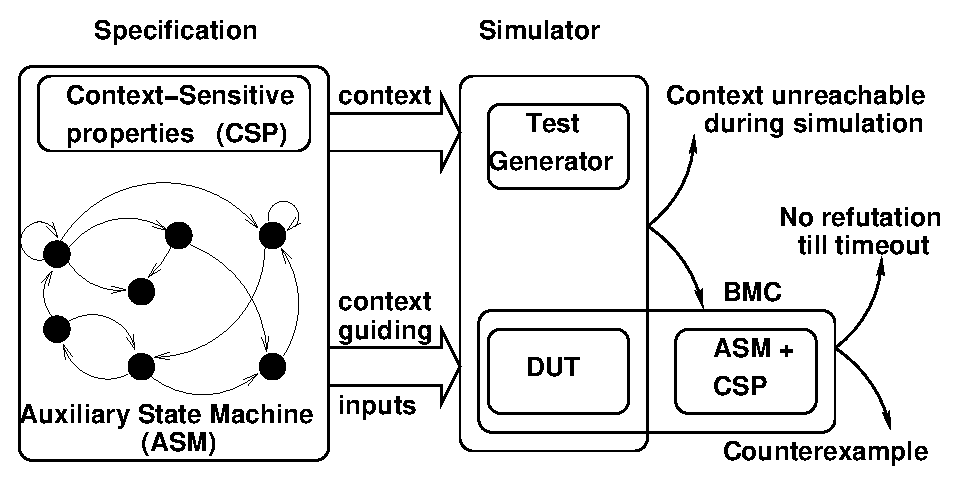
\includegraphics[scale=0.66]{diag4.eps}
\caption{Proposed Architecture} \label{fig3.1}
\end{figure}

Figure~\ref{fig3.1} shows the approach adopted in this work.
\begin{enumerate}

\item In the first step, we use the auxiliary state machines to guide
    a semi-formal simulation engine in generating test inputs 
	that can guide the DUT towards the context-satisfying
    states. We treat the DUT as a black-box and co-simulate the
    auxiliary state machines with the DUT. Since the auxiliary state
    machines contain both input and output signals of the DUT, this
    step is a game between the DUT and the simulation test-bench, where the
    test-bench wins if a context-satisfying state is reached.

\item Once a context-satisfying state is reached, we use BMC to verify
    the given context sensitive property from that state.

\end{enumerate}

\noindent
The algorithms behind each of the above steps is given in the thesis. 
In Step 1, the test generator is built as an {\em oracle} along similar ideas 
as presented in Section~\ref{sec4}. At each simulation cycle, this oracle 
examines the current context, and attempts to generate an input assignment 
that has the best possibility to guide the DUT towards the target context. 
To give an idea of the working of our procedure, we present the following 
example.

\begin{example} \label{eg5}
{\em Consider property ${\cal P}_0$ of Example~\ref{eg1}.
The context of this property is $WAIT$. Consider a DUT implementing 
the master. In Step 1 above, the idea is to analyze the auxiliary state 
machine and drive simulation inputs 
that guide the DUT towards the $WAIT$ context. $gnt$ is an
input to the master, hence, the test generator drives $gnt$.
Initially, the master is idle with $req=0$. The initial context of 
the DUT is $IDLE$.

In the first cycle, the oracle examines the current
context $IDLE$ of ${\cal M}1$ and the target context $WAIT$ and chooses
the transition $(IDLE, WAIT)$ since this leads to a state that is closest 
to the target $WAIT$ context. The condition enabling this transition
is $req \land \neg gnt$, and hence, the oracle returns the input
constraint $gnt=0$. For the other input signals $rdy$ and $abort$, the test
generator makes a random assignment. It may be noted that had the oracle
taken $gnt=1$, there was a possibility of the DUT being driven towards
the $INIT$ context (depending on the DUT response), which is further
away from the $WAIT$ context. However, the oracle avoids such
possibilities.

The DUT and ${\cal M}1$ are now co-simulated with a random input vector with
$gnt=0$ as the input
bias, and the DUT response is sampled. The next context is determined
by the combined choice of the test-bench (gnt = 0) and the DUT response.
In case the DUT assigns $req$ to 0, the context remains
$IDLE$, while it goes to $WAIT$ if it chooses $req=1$. This process continues
till we reach a state satisfying the context, or we reach end of
simulation.

It may be noted that there is no guarantee that our intelligent test
generator will always be able to force the DUT to the $WAIT$ context. For
example, consider a DUT that never asserts the $req$ signal. In such a
case, the context after every co-simulation step remains
$IDLE$.
} $\Box$
\end{example}

\subsubsection{Implementation and Results} \label{sec5.3.1}
To demonstrate the 
efficacy of our proposed semi-formal methodology, we implemented our 
algorithm on top of two popular verifiers, namely Magellan~\cite{magellan} 
from Synopsys and VIS~\cite{vis}. We analyzed the advantages of our approach 
on several verification IPs for standard Bus protocols.
Our methodology produced (a) results of 
higher simulation coverage in lesser time as compared to coverage driven 
randomized test benches, and (b) lesser memory requirement as
compared to a purely formal methodology. Below, we present a snapshot of the 
results obtained using Magellan.

\begin{table*}[htb]
\begin{center}
{\small
\begin{tabular}{|c|c|c|c|c|c|c|c|c|c|} \hline
Ckt. & \#Inp. & \#OutP. & \#Seq. & \#Comb & \#Nets & Rand. & Formal & Our \\
Module & & & & & & Sim & Engine & Approach \\ \hline \hline
Coherence P1 & 69 & 6 & 304 & 3750 & 4123 & 1899 & 2499 & 489 \\ \hline
Coherence P2 & '' & '' & '' & '' & '' & 899 & 1449 & 589 \\ \hline
PCI P1 & 162 & 207 & 3802 & 26424 & 30388 & 2349 & 1649 & 349\\ \hline
PCI P2 & '' & '' & '' & '' & '' & timeout & 3649 & 1149 \\ \hline
\end{tabular}
}
\end{center}
\caption{Simulation Cycle Comparison} \label{tab3}
\end{table*}

Table~\ref{tab3} shows the results of different experimentations with
Magellan, run in different modes. The designs used in our work consists
of circuit modules from~\cite{open, texas}. 
Columns 2 to 6 present the design statistics
generated by Magellan. The seventh column
shows the number of simulation cycles required by Magellan when
run in random simulation mode, while the next column shows the
corresponding number when the purely formal engine mode is invoked.
In both the cases, the auxiliary state machines are added to
the RTL and Magellan checks
for violation/success of the assertion on the product of the DUT and the
auxiliary machines.
Timeout indicates that the property was not covered even after
10,000 cycles.
In our implementation scheme, the auxiliary state
machine is coded as a simulation input bias in the first phase, while
it is considered as part of the RTL in the second stage.
The final column shows the number of simulation cycles when Magellan is
run as per our implementation scheme.
Results show the efficacy of our approach in terms of simulation
cycles.

\subsection{Context Sensitive Properties: Consistency Analysis} \label{sec5.4}
The main motivation of this work was to develop consistency analysis 
procedures for this style of formal specifications consisting of auxiliary 
state machines and context-sensitive formal properties. In particular, 
we analyzed the satisfiability and realizability problems
and showed that the complexities of these procedures are 
same as in the case of normal LTL (PSPACE-complete and 2-EXPTIME-complete 
respectively). This is good news, since this allows
us to develop arbitrarily complex auxiliary state machines to facilitate 
the process of formal specification development without
any exponential blow-up in the complexity of consistency checking 
procedures.

The more important contribution of this work was to show that 
the complexity of {\em realizability} checking of 
a rich fragment of this mixed specification language is EXPTIME-complete. 
In particular, this fragment restricts context-sensitive properties 
to the GR(1)~\cite{nir} subset of LTL, while the definition 
of the auxiliary state machines remain as earlier. 
This can significantly extend the expressive power of GR(1) LTL beyond simple
Streett~\cite{nir} requirements, thereby, making it more practical and useful.

The main highlight of our approach was to establish that a
formal specification consisting of auxiliary state machines and
GR(1) LTL properties is also contained in the GR(1) subset of LTL, and
therefore, has a lower realizability checking complexity.

\section{Open Linear Temporal Logic for modular FPV} \label{sec6}
In view of the inherent capacity limitation of FPV techniques, there has 
been a paradigm shift from a system level validation perspective to a 
modular validation one. A design typically consists of a set of interacting 
modules. The validation
task in this new perspective amounts to verifying each module in
isolation (module checking) and then verifying their interaction protocols.

A module is an open system which interacts with its environment
and whose behavior depends on this interaction. The environment of a module
consists of the responses of its peer modules with which it interacts through
its interface. Validating the module against all possible valid environments
is again an explosive task. In reality, only a subset of the possible
environments needs to be modeled on the basis of the environment interactions
which can affect the module behavior. The main challenge in modular 
verification lies in modeling this interaction. 
Researchers have studied a few approaches for modeling the 
module-environment interaction. One approach~\cite{alfaro} defines 
an interface
process (an interface of a module consists of its input-output behavior)
and verifies a module in isolation by composing the module
behavior with its interface. The interface process mimics the behavior of the
environment of the module and thus the desired verification task is
accomplished. In a second approach~\cite{josko1}, for each module, the original
specification is partitioned into the assume and the guarantee
and the module is checked to determine whether it satisfies the guarantee
in presence of the assumptions, and a composition rule is defined to compose
the verification tasks for each module to reason about the entire system.
However, both the above approaches are non-trivial. The
construction of the interface process is difficult in the former approach while
the latter approach is non-trivial due to the inherent intricacy involved
in assume-guarantee separation of the specification.

In our work, we have proposed a new style of modeling this interaction. 
Our motivation was the fact that formal property 
specification languages like Computation Tree Logic (CTL) or Linear Temporal 
Logic (LTL) were originally developed for closed systems. These languages, 
therefore, do not lend themselves
easily to the specification of behaviors of open systems, and thereby, 
give rise to several semantic problems, as we first explain below. This 
motivated us to propose the new specification language.
To elaborate our views, we consider two of the most sensitive issues in
open system specification, namely those of {\em realizability}~\cite{rosner}
and handling of negation.

\subsection{The Realizability Problem due to absence of input-output 
	discrimination} \label{sec6.1}
Existing temporal logics do not distinguish between input and output 
variables, and thereby permit properties, that are unrealizable for 
open systems. Consider the LTL
property for an arbiter module ${\cal M}$ with $req$ as input and $gnt$ as
output:
\[  G[\ gnt\ \Rightarrow\ X \neg req\ ] \]
The property attempts to express the requirement that the $req$ line should
be de-asserted in the cycle following a $gnt$. The arbiter ${\cal M}$ can
never {\em guarantee} $X \neg req$ after asserting a $gnt$ because $req$ is
asserted by another device. Actually the property should be checked on the
device that asserts the $req$, but current property checkers
do not have any syntactic means to prevent the designer from checking
this property on the arbiter.

\subsection{Issue of Negation} \label{sec6.2}
\noindent
Consider the following LTL property for an arbiter:
\[ P1: \qquad req\ \Rightarrow\ X gnt \]
which says: {\em the output $gnt$ is asserted in the cycle following the
receipt of input $req$}. When we consider the negation of $P1$,
we are often interested in checking whether the path satisfies
$req$, but not $X gnt$. The truth of the property (or its negation) on paths
that do not have any $req$ at all are of no relevance. 
Logical negation does not achieve this
objective. The negation of $P1$ is:
\[ P1': \qquad req\ \land \neg X gnt \]
which is false on paths that do not have any $req$ at all. As a result, the
negated property $P1'$ is unrealizable, since the arbiter can never guarantee
that $req$ will be asserted.

\subsection{Open Linear Temporal Logic: A new solution} \label{sec6.3}
\noindent
In our work, we propose a new style for writing temporal specifications 
in LTL for open systems that helps the designer to avoid specification 
inconsistencies described above.
The main focus of this was to show that a syntactic distinction between
the input variables and the state variables in a property for a module helps
in avoiding realizability problems arising due to lack of input-output 
discrimination. In Open-LTL, the temporal operators,
namely $X$ (next-time) and $U$ (until), are
annotated with constraints over input variables 
and the property itself is defined only over the
state propositions of the module. This extension yields a 
logic derived out of Linear Temporal Logic (LTL). We call this new logic
{\em Open Linear Temporal Logic} (Open-LTL).

\noindent
The semantics of our proposed extensions follow from the assume
guarantee style of reasoning~\cite{henzinger}. For example, the Open-LTL
property $f\ U_{I}\ g$
is true if the LTL property $f\ U\ g$ holds on the runs where the environment
presents inputs satisfying the input constraint $I$ along the run. This 
discrimination between inputs and output variables helps us in avoiding 
the semantic anomalies, as discussed below.
For example, the property
$G[\ o\ \Rightarrow\ X i\ ]$ is not allowed as a property to be
checked on the module having input $i$ and output $o$, but can be expressed 
for the device having input $o$ and output $i$ as:
\[ G[\ X_{o}\ i\ ] \]
In Open-LTL, we interpret negation in the {\em assume-guarantee} sense. We will
express $P1$ as $X_{req}\ gnt$, and interpret its negation as:
\[ \neg X_{req}\ gnt = X_{req}\ \neg gnt \]
Note that the negation applies on the {\em guarantee}, while the {\em assume}
(namely, $req$) remains the same. Interpreting this semantics over a path,
we find that $P1$ is true when $gnt$ is asserted after a $req$, and the
negation of $P1$ is true when $gnt$ is not asserted after a $req$. When
$req$ is not asserted, both properties are vacuously true.

The formal syntax and semantics of Open-LTL are given in the thesis. We 
illustrate its application on a simple example below.

\begin{figure}[htb]
\psfrag{ni2}{$\bf \neg i_2$}
\psfrag{I=i1&ni2}{$I=i_1 \land \neg i_2$}
\psfrag{I=i1&ni2}{$I=i_1 \land \neg i_2$}
\psfrag{i1}{$\bf i_1$}
\psfrag{i2}{$\bf i_2$}
\psfrag{ni1}{$\bf \neg i_1$}
\psfrag{ni12}{$\bf \neg (i_1 \land i_2)$}
\psfrag{ni1ni2}{$\bf \neg (i_1 \lor i_2)$}
\psfrag{i1ori2}{$\bf i_1 \lor i_2$}
\psfrag{i1i2}{$\bf i_1 \land i_2$}
\psfrag{ni1i2}{$\bf \neg i_1 \land i_2$}
\psfrag{i1ni2}{$\bf i_1 \land \neg i_2$}
\centering
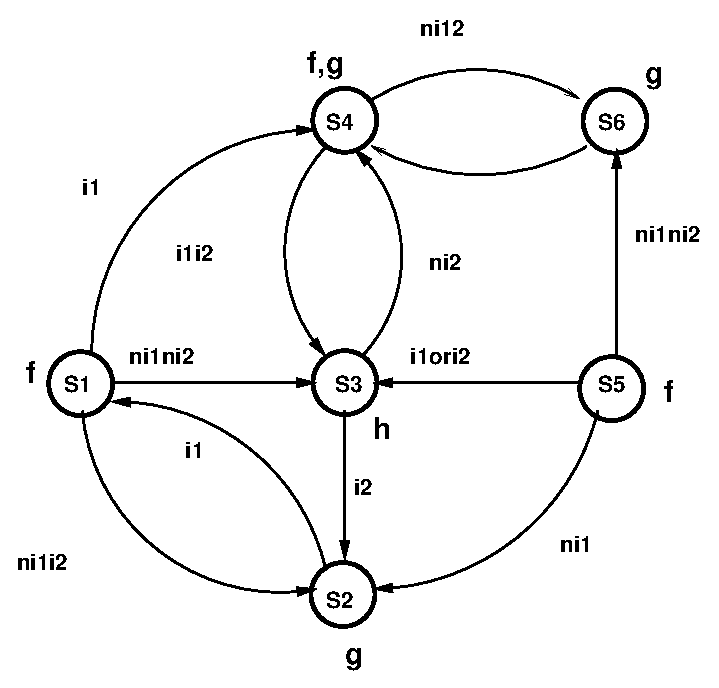
\includegraphics[scale=0.75]{diag31.eps}
\caption{A Simple Module} \label{Fig1}
\end{figure}

\begin{example}
{\em
Figure~\ref{Fig1} shows a simple module with the set of states 
$S =$  \{S1, S2, S3, S4, S5, S6 \},
{\cal AP} = \{ $f, g, h$\} and $\mathbb{I}$ = \{ $i_1, i_2$ \}.
The set of input vectors enabling each transition is shown as a Boolean
function beside the transition. For example, the transition from
$S1$  to  $S4$ is
enabled by two input vectors, namely $\eta{_1}$ = (1,0) and $\eta{_2}$ = (1,1)
which are collectively represented by the Boolean formula $i_1$.
Let us consider the following Open-LTL formula:
\[ \varphi  =  f\  U_{\cal I}\  g \]
where ${\cal I} = i_1 \land \neg i_2$. From $S1$, the input
constraint ${\cal I}$
enables only the transition to $S4$ (which satisfies $g$), and therefore
$\varphi$ is true at $S1$. On the other hand, from state $S5$, the only
transition enabled by ${\cal I}$ is the one to $S3$, and hence $\varphi$ is
false at $S5$. Since $g$ is true in the states
$\{S2, S4, S6\}$, $\varphi$ is true at these states. Since $S3$
does not satisfy $f$, $\varphi$ is false there.

Let us now suppose that ${\cal I} = \neg i_1$ in $\varphi$. From $S1$,
${\cal I}$ enables the transitions to $S3$ and $S2$. Since $g$ does not
hold at $S3$, therefore $\varphi$ is false at $S1$.
Similarly, from $S5$, ${\cal I}$ enables the transitions to $S6$ and $S3$.
To see
that ${\cal I}$ enables the transition from $S5$ to $S3$, consider the
fact that this transition is enabled by three input vectors, namely,
$\eta_0 = (0,1)$, $\eta_1 = (1,0)$ and $\eta_2 = (1,1)$.
Since $\eta_0$ satisfies ${\cal I} = \neg i_1$, the transition from
$S5$ to $S3$ is enabled. Therefore, $\varphi$ is false at $S5$ (by
virtue of the path through $S3$).
} $\Box$
\end{example}

\subsection{Verification Algorithms} \label{sec6.4}
\noindent
We have proposed a symbolic model checking method for checking
Open-LTL properties on a given module. The algorithm is similar to the
classical tableau method for LTL model checking~\cite{clarke:00}, with 
some modifications to handle the input constraints. The input constraints 
were used to prune the module, and thereby, resulted in a
significant space advantage.

We implemented a prototype model checker for Open-LTL. To demonstrate 
the efficacy of our approach towards modular validation, we 
experimented with several benchmark circuits and got dramatic 
improvements in performance in terms of space. This is primarily 
because our approach 
verifies modules in isolation with respect to a set of relevant input 
scenarios captured as input constraints in the property. A detailed 
analysis of the results appears in the thesis.

\section{An integrated framework for ABV for UML Statecharts} \label{sec7}
For quite some time, the Unified Modeling Language (UML) has been
adopted by designers of safety critical control systems such as
automotive and aviation control. This has led to an increased emphasis
on setting up a validation flow~\cite{room} over UML that can be used to 
guarantee the correctness of UML models.

In view of the capacity limitations of FPV techniques, a dynamic ABV 
validation approach seems to be a natural choice.
The main contribution of this work was to formalize and develop a dynamic 
ABV platform for verifying behavioral properties of communicating
concurrent systems described using UML Statecharts. Our idea was 
developed on top of Rhapsody~\cite{rhap}, one of the most popular 
tools for model-based development using UML. 

The development of the ABV platform posed two main non-trivial challenges.
These are as follows:

\begin{itemize}

\item {\em Choice of an assertion specification language:} The language 
	should be rich enough to support correctness requirements arising in
    software systems.

\item {\em Architecting the ABV engine:} Building the ABV algorithm on top 
	of Rhapsody was a challenge, and required a sound understanding of 
	the semantics of Statechart simulation, as employed in the tool.

\end{itemize}

\noindent
In the subsequent discussion, we briefly describe our solutions to 
each of the above.

\subsection{Assertion Specification Language} \label{sec7.1}
To describe correctness properties for UML models, one needs to 
describe properties over data attributes and events as well.
Property specification languages that have been widely used in
the property verification community are pre-dominantly either
state-based or event-based. However, for our purpose, we need
to specify both {\em state} information and events (communication
among components). For example, the Local Interconnect Network
(LIN)~\cite{lin} protocol specification has the following requirement:
{\em In slave node, detection of break/synch frame shall abort
the transfer in progress and processing of the new frame shall
commence}. As this shows, both states (for describing a transfer in progress)
and events (break/synch event) are required to
capture the desired behavior. A more formidable 
challenge is to define the semantics of the property specification 
language in the absence of the clock (unlike in hardware). 

To address the above issue, we extended Linear
Temporal Logic (LTL) with some interesting features, specifically,
the ability to express requirements over events, ability to express
arithmetic and relational queries over data attributes, 
the concept of local variables and the concept of
parameterized events. Our logic is called Action-LTL and is used
within our ABV framework for specifying assertions. 

The idea of combining state-based and event-based formalisms for the
verification of systems is not new, and several specification paradigms have
been proposed over the past few years.
A detailed discussion of the different approaches in combining states and
events for property specification can be found in~\cite{chaki1}. 
However, the support for local variables and parameterized events 
are new in Action-LTL. 
The additional novelty of Action-LTL lies in its semantics, which had to be 
defined in accordance to the 
simulation semantics of Rhapsody, and was therefore, a non-trivial task. 
The syntax and semantics of Action-LTL appears in the thesis. 
Below, we present a couple of representative properties for the Local 
Interconnect Protocol (LIN)~\cite{lin} encoded in Action-LTL. 
The variables that begin with the prefix {\em ev} represent events.

\begin{itemize}

\item ${\cal P}_1$: G[(Slv.FrmType == UNCONDITIONAL) 
	$\Rightarrow$(Slv.PID $\ge$ 0x00 $\land$ Slv.PID $\le$ 0x3b)]: This 
	property formally expresses the requirement that unconditional frames 
	always carry signals and their identifiers are in the range 0 to 59(0x3b).
\item ${\cal P}_2$: G[(Slv.state == Active) $\land$ Slv.evBrkSync 
	$\Rightarrow$ (Slv.state == RcvPID)]: This property formally expresses 
	the requirement that in a slave node, detection of break/synch event 
	shall abort the transfer in progress and processing of the new frame 
	shall commence.
\end{itemize}

\begin{figure}[htb]
\centering
\includegraphics[scale=0.6]{uml.pstex}
\center
\caption{The ABV platform over Rhapsody} \label{fig5.1}
\end{figure}

\subsection {Architecting the ABV engine} \label{sec7.2}
The ABV engine was built on top of Rhapsody, using the standard concept 
of dynamic property monitoring over simulation runs as explained in 
Subsection~\ref{sec2.2}. This posed several non-trivial challenges, starting 
from accessing the interface signals to creation and integration of 
assertion monitors, and required us to engineer the internals of Rhapsody 
to implement the algorithms. In addition, we embedded the concept of 
property guided simulation inside our ABV framework using the idea presented in Section~\ref{sec4}. 

Figure~\ref{fig5.1} shows the overall architecture. This tool was successfully 
used to verify an industrial implementation of the LIN protocol in UML.
We believe the successful deployment of ABV over Rhapsody achieved by us 
in this work will open up the avenue for future research on ABV for 
more generic software validation.

\section{Organization of the dissertation} \label{sec8}
The thesis is organized into 9 chapters. A summary of the contents of the
chapters is as follows:

\begin{description}
\item {\bf Chapter 1}: This chapter contains an introduction and a summary
of the major contributions of this work.

\item {\bf Chapter 2}: A detailed study of the background concepts required 
for this thesis and a survey of relevant research is presented
here.

\item {\bf Chapter 3}: This chapter describes the concept of 
property guided simulation for ABV.

\item {\bf Chapter 4}: This chapter formalizes the concept of auxiliary 
state machines and context-sensitive formal specifications, and 
presents the algorithm for FPV.

\item {\bf Chapter 5}: This chapter describes the idea of semi-formal 
verification of Subsection~\ref{sec5.3}. 

\item {\bf Chapter 6}: This chapter describes the work on consistency 
analysis described in Subsection~\ref{sec5.4}.

\item {\bf Chapter 7}: This chapter presents the work on Open Linear Temporal 
Logic.

\item {\bf Chapter 8}: This chapter presents the work on the development 
of the ABV platform for UML Statechart validation.

\item {\bf Chapter 9:} We summarize with conclusions on the contributions of 
this dissertation.

\end{description} 

\newpage
\section{Dissemination of this work} \label{sec9}
\begin{enumerate}

\item Banerjee, A., Dasgupta, P., and Chakrabarti, P.P., Realizability of 
	Auxiliary State Machines + GR (1) LTL, To Appear in VDAT 2007.

\item Banerjee, A., Dasgupta, P., and Chakrabarti, P.P., 
	Can Semi-Formal be made more Formal? In Proc. of GMISL Symposium, 
	January 2007.

%\item Banerjee, A., Dasgupta, P., and Chakrabarti, P.P., 
%	Formal Methods for Checking Realizability of Coalitions 
%	in 3-party Systems, In Proc. of MEMOCODE 2006, pp. 

\item Banerjee, A., Pal, B., Das, S., Kumar, A., and Dasgupta, P., 
	Test Generation Games from Formal Specifications, In Proc. of 
	Design Automation Conference (DAC) 2006, pp. 

\item Banerjee, A., and Dasgupta, P., The Open Family of Temporal Logics: 
	Annotating Temporal Operators with Input Constraints, In Proc. of ACM 
	Transactions on Design Automation of Electronic Systems (TODAES), 
	July 2005, pp. 492-522.

\item Banerjee, A., Pal, B., Dasgupta, P., Chakrabarti, P.P., Jha, M., and 
	Cerny, E., Design Issues for Assertion-Based Verification IPs: The 
	OVA Experience, In Proc. of SNUG 2004.

\item Banerjee, A., Dasgupta, P., and Chakrabarti, P.P., Auxiliary State 
	Machines + Context-Sensitive Formal Properties in Formal 
	Verification, {\em Communicated to} ACM TODAES.

\item Banerjee, A., Dasgupta, P., and Chakrabarti, P.P., Semi-Formal 
	Verification with Auxiliary State
    Machines + Context-Sensitive Formal Properties, 
	{\em Communicated to} IEEE TCAD.

%\item Banerjee, A., and Dasgupta, P., Realizability of Temporal Logic 
%	Specifications, Preliminary Acceptance in {\em Handbook of Research on 
%	Modern Systems Analysis and Design Technologies and Applications}. 

\item Pal, B., Banerjee, A., Sinha, A., and Dasgupta, P., Accelerating 
	Assertion Coverage with Adaptive Test-benches, 
	{\em Communicated to} IEEE TCAD.

\end{enumerate}

\newpage
{\footnotesize
\begin{thebibliography}{99}

\bibitem {abraham}  Abraham, J.A., Vedula, V.M., and
          Saab, D.G., Verifying Properties Using Sequential
          ATPG; In ITC 2002, pp. 194-202.

\bibitem {alfaro}  Alfaro, L. de, Henzinger, T., 
          Interface Automata, In Ninth Annual Symposium on Foundations 
	  of Software Engineering, ACM Press, 2001, pp. 109-121.

\bibitem{alur-ltl} Alur, R., and Torre, L., S., Deterministic 
	Generators and games for LTL fragments, In ACM Trans. Comput. 
	Logic 2004, 5(1), pp.1-25.

\bibitem{Alur:93} Alur, R., Courcoubetis, C. and Dill, D.L.,
        Model Checking in dense real-time.
        {\em Information and Computation}, 104(1):2-34, 1993.

\bibitem{Alur:94} Alur, R. and Henzinger, T.A.,
         A really temporal logic,
         {\em Journal of the Association for Computing Machinery}, 41(1):
         181-204, 1994.

\bibitem {ammann} Ammann, P.E., Black, P.E., and Majurski, W.,
        Using Model Checking to Generate Test from Specifications; In
        ICFEM 1998, pp. 46-54.

\bibitem{ahb} {\em ARM AMBA Specification Rev 2.0}, http://www.arm.com 

\bibitem{vmm} Bergeron, J., Cerny, E., Hunter, A., and
    Nightingale, A., {\em Verification Methodology Manual for System
    Verilog}, Springer Verlag, 2005.

\bibitem{bmc} Biere, A., Cimatti, A.,  Clarke, E.M., and Zhu, Y.,
    Symbolic Model Checking without BDDs, LNCS 1579, pp. 193-207, 1999. 

\bibitem{chaki1} Chaki, S., Clarke, E., Ouaknine, J., Sharygina, N.
    and Sinha, N.,
    Concurrent software verification with states, events, and deadlocks,
    Formal Aspects of Computing 17(4), 2005, pp. 461-483.

\bibitem{ctl}  Clarke, E.M., Emerson, E.A., and Sistla, A.P., Automatic
        verification of finite-state concurrent systems using temporal logic
        specifications, {\em ACM Trans. on Prog. Lang. and Systems},
        8(2):244-263, 1986. 

\bibitem{clarke:00a} Clarke, E., German, S., Lu, Y., Veith, H., and Wang, D.,
        Executable Protocol Specification in ESL;
        FMCAD'00, 197-216. 

\bibitem{cav} Clarke, E.M.  and Kurshan, R.P.
        {\em Computer Aided Verification}, IEEE Spectrum, 33(6):61-67. 

\bibitem{clarke:00} Clarke, E.M., Grumberg, O., and Peled, D.A.,
        {\em Model Checking}, MIT Press, 2000.

\bibitem{dam} Dams, D., {\em Abstract Interpretation and Partition Refinement 
	for Model Checking,} PhD thesis, Technical University of Eindhoven, 
	1996.

\bibitem{pdgbook} Dasgupta, P., A Roadmap for Formal Property Verification,
        Springer, 2006. 

\bibitem{dill} Dill, D.L., {\em Trace Theory for Automatic Hierarchical
        Verification of Speed-independent Circuits.} ACM Distinguished
        Dissertations. MIT Press, 1989.

\bibitem{Emerson:89} Emerson, E.A., Mok, A.K., Sistla, A.P., and
    Srinivasan, J., Quantitative temporal reasoning, In {\em Proc. of
	Real Time Systems}, 4(4):331-352, 1992.

\bibitem{garg} Gargantini, A., Heitmeyer, C.,
    Using Model Checking to Generate Tests from Requirements
    Specifications; SIGSOFT'99, pp. 146-162.

\bibitem{approx} Govindaraju, S.G., and Dill, D.L., Verification by
    approximate forward and backward reachability. In {\em Proc. of
    Int. Conf. on Computer Aided Design} (ICCAD), pp. 366-370, 1998. 

\bibitem{SAT:01} Gupta. A.,Casavant. A.E.,Ashar P., and Liu X.G.,
         Property Specific Testbench Generation for Guided Simulation;
         In VLSI/ASPDAC 2002, pp. 524-534.

\bibitem{henzinger} Henzinger, T., Qadeer, S., and Rajamani, S.,
        Decomposing Refinement Proofs using Assume-Guarantee Reasoning,
        In Proceedings of ICCAD, pp. 245-252, 2000.

\bibitem{grumberg:94} Grumberg, O., and Long, D.E., Model Checking and
    Modular Verification, {\em ACM Trans. on Prog. Lang. and Systems},
    16, pp. 843-872, 1994.

\bibitem{ibm} IBM CoreConnect,
        http://www-306.ibm.com/chips/techlib/techlib.nsf/techdocs 

\bibitem{barbara} Jobstmann, B., and Bloem, R., Optimizations 
	for LTL synthesis, FMCAD 2006, pp. 117-124.

\bibitem{josko1} Josko, B., MCTL - an extension of CTL for modular
        verification of concurrent systems,
        In Proceedings of {\em Temporal Logic in Specification} LNCS, vol.
        398, Springer Verlag, pp. 165-187, 1987.

\bibitem{lily} Lily: A Linear Logic Synthesizer, 
	http://www.ist.tugraz.at/staff/jobstmann/lily

\bibitem{lin} Local Interconnect Network, http://www.lin-subbus.org/

\bibitem{magellan} Magellan - Hybrid RTL Formal Verification, 
        http://www.synopsys.com/products/magellan/

\bibitem{mc} McMillan, K.L., Symbolic Model Checking, Kluwer Academic 
	Publishers, 1993.

\bibitem{kunz} Nguyen, D. M., Stoffel, D., Wedler, M., and
        Kunz, W., Transition-by-Transition FSM Traversal
        for Reachability analysis in Bounded Model Checking,
        In ICCAD 2005, pp. 1060-1067. 

\bibitem{uml} Object Management Group, {\em Unified Modeling
    Language Specification}, Version 1.4, Draft, OMG(2001),
    http://cgi.omg.org/cgibin/docad/018214.

\bibitem{open} OpenCores, http://www.opencores.org/

\bibitem{pci} {\em PCI Local Bus Specification Revision 2.2},
        http://www.pcisig.com/specifications/conventional.

\bibitem{nir} Peterman, N., Pnueli, A., and Sa'ar, Y.,
    Synthesis of Reactive(1) Designs, In Conference on
    Verification, Model Checking and Abstract Interpretation,
    pp. 364-380, 2006.

\bibitem{psl} Property Specification Language, http://www.eda.org/ieee-1850 

\bibitem{pnueli:77} Pnueli, A., The temporal logic of programs,
        In {\em Proceedings of 18th Foundations of Computer Science},
        1977, pp. 46-57.

\bibitem{rosner} Pnueli, A., Rosner, R., On the Synthesis of a Reactive Module,
        In Principles of Programming Languages (POPL), 1989, pp. 179-190.

\bibitem{soc} Rashinkar, P., Paterson, P., Singh, L.,
    SYSTEM-ON-A-CHIP VERIFICATION Methodology and Techniques,
    Kluwer Academic Publishers.

\bibitem{rvm} Reference Verification Methodology for Vera, \\
    http://www.synopsys.com/products/simulation/pdf/va\_vol4\_iss1\_vera.pdf

\bibitem{room} Selic, B., Gullekson, G., and Ward, P., Real-Time
    Object-Oriented Modeling. John Wiley \& Sons, Inc., 1994.

\bibitem {dill1} Shimizu, K., and Dill, D.L., Deriving a simulation input
        generator and a coverage metric from a formal specification, In
        Proceedings of DAC 2002, pp. 801-806.

\bibitem{guido} Shyam, S., and Bertacco, V., Distance-Guided
        Hybrid Verification with GUIDO, In DATE'2006, pp. 1211-1216.

\bibitem{synopsys_beh} Synopsys Behavioral Compiler,
        $http://www.synopsys.com/products/beh\_syn/beh\_syn.html$

\bibitem{dc} Synopsys Design Compiler,
    $http://www.synopsys.com/products/logic/design\_compiler.html$

\bibitem{synopsys} Synopsys Physical Design Tools,
        http://www.synopsys.com/sps/phydes.html

\bibitem{sva} System Verilog.
        http://www.systemverilog.org/

\bibitem {tasiran} Tasiran, S., Yuan, Y., Batson, B., Using a formal
        specification and a model checker to monitor and direct
        simulation, In Proceedings of DAC 2003, pp. 356-361.

\bibitem{texas} {\em Texas-97 Verification Benchmarks},
    http://www-cad.eecs.berkeley.edu/Respep/Research/vis/texas-97/

\bibitem{rhap} The Rhapsody UML Verification Environment, 
	http://www-omega.imag.fr/doc/d1000312\_1/WP22-312-V1-ruve2004.pdf 


\bibitem{vardi} Vardi, M.Y., and Wolper, P., An automata-theoretic approach
    to automatic program verification. In {\em Proc. of Logic in Computer
    Science} (LICS), 1986.

\bibitem{vcs} VCS,
    http://www.synopsys.com/products/simulation/simulation.html 

\bibitem{vis} VIS Homepage, http://vlsi.colorado.edu/$\sim$vis 
\end{thebibliography}
}

\end{document}
